\chapter{代数拓扑}
    \section{Brouwer不动点定理与Sperner引理}
    我们首先叙述 Brouwer不动点定理与Sperner引理:
    \begin{theorem}[Brouwer不动点定理]
        设 $f$ 是 $n$ 维闭球 $B^n$ 到自身的连续映射, 则 $f$ 必有不动点.
    \end{theorem}
    \begin{lemma}[Sperner引理]
        设 $K=[v_0,\dots,v_n]$ 是 $n$ 维单纯形, 考虑其三角剖分 $T$, 将 $T$ 的顶点 $(n+1)$ 染色, 即定义 $\lambda:V(T)\rightarrow\{0,\dots,n\}$, 且满足对任意指标子集
        $\{i_0,\dots,i_k\}\subseteq\{0,\dots,n\}$, $\lambda$ 在 $[v_{i_0},\dots,v_{i_k}]$ 上的限制的值域包含于 $\{i_0,\dots,i_k\}$. 则一定存在 $u_0,\dots,u_n\in V(T)$, 
        使得 $[u_0,\dots,u_n]$ 是三角剖分 $T$ 的单形, 且 $\lambda(u_i)$ 互不相同.
        \begin{figure}[hbtp]
            \centering
            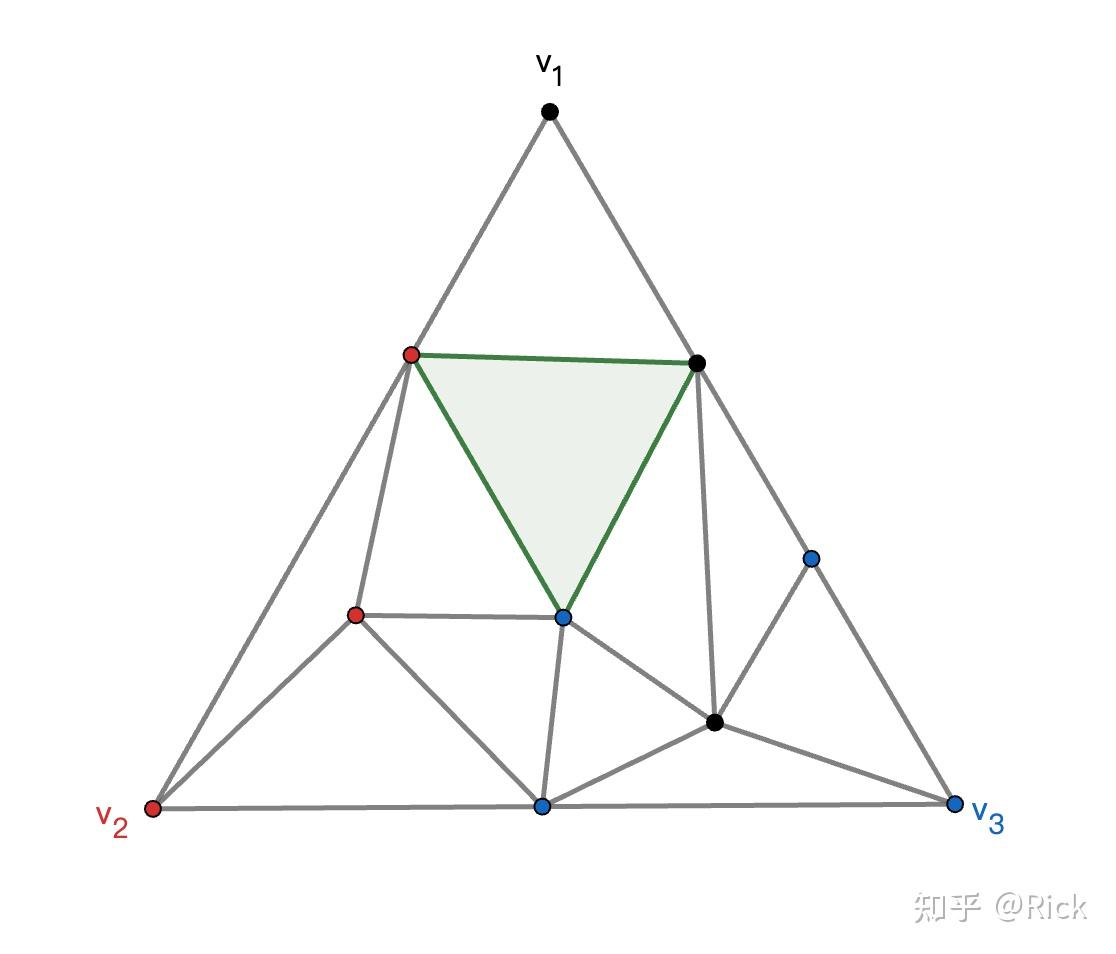
\includegraphics[scale=0.2]{Figures/SpernerLemma.jpg}
            \caption[SpernerLemma]{Sperner引理示意图}
        \end{figure}
    \end{lemma}

    它们一个是拓扑的定理, 一个是组合的定理, 看似没有联系, 但实际上我们能证明它们是等价的: 由于 $B^n\cong K$, 我们将 Brouwer不动点定理的叙述改为 $K$ 到自身的连续映射 $f$ 必有不动点.

    $1^{\circ}$:Sperner引理 $\Rightarrow$ Brouwer不动点定理
    
    设 $K = [v_0,\dots,v_n]$ 是 $n$ 维单形, 对 $\forall x\in K$, $x=\sum_i\alpha_iv_i,\,\alpha_i\geqslant0,\,\sum_i\alpha_i=1$. 设 $f(x) = \sum_i\beta_iv_i$, 定义染色映射 
    $\lambda(x)$ 为使得 $\alpha_i\geqslant\beta_i$ 且 $\alpha_i\neq0$ 的最小下标 $i$. 我们首先观察到在任意集合 $\{i_0,\dots,i_k\}\subseteq\{0,\dots,n\}$ 中, 
    对 $\forall x\in[v_{i_0},\dots,v_{i_k}]$, $x$ 的坐标 $\alpha$ 满足 $\alpha_i=0,\,i\notin\{i_0,\dots,i_k\}$, 因此 $\lambda(x)$ 只可能在 $\{i_0,\dots,i_k\}$ 中取值.

    固定染色 $\lambda$, 取重心重分 $K^0,K^1,\dots$, 则在每一个 $K^j$ 中 $\lambda$ 均满足引理条件, 于是存在异色单形 $\Delta^j=[u^j_0,\dots,u^j_n]$, 不妨设 $\lambda(u^j_i)=i$.
    因为 $K$ 是紧集, 因此 $\{u^j_0\}_j$ 存在收敛子列, 不妨设就为序列本身, 由重心重分的性质知 $\Delta^j$ 的直径趋于零, 因此对所有 $i$, $\{u^j_i\}_j$ 均收敛于同一点 $u$, 即 
    $u=\lim\limits_{j\rightarrow\infty}u^j_i,\,\forall\,i=0,\dots,n$. 由染色的定义知 $u^j_i$ 的 $v_i$ 坐标不等于零且大于等于 $f(u^j_i)$ 的, 
    根据极限的保号性知 $u$ 的所有坐标 $\alpha_i$ 大于等于 $f(u)$ 对应的坐标 $\beta_i$, 但因为 $\sum_i\alpha_i = \sum_i\beta_i = 1$, 所以 $\alpha_i=\beta_i$, 因此 $u = f(u)$ 是 $f$ 的不动点.

    $2^{\circ}$:Sperner引理 $\Leftarrow$ Brouwer不动点定理
    
    设 $K = [v_0,\dots,v_n]$ 是 $n$ 维单形, $\lambda$ 为满足引理要求的染色, $T$ 是 $K$ 的一个三角剖分, 则可以定义单纯映射 $f:K\rightarrow K$ 如下: 对 $\forall x\in V(T)$, 
    定义 $f(x) = v_{\lambda(x)}$, 若 $x = \sum_{i=0}^{k}\alpha_ix_i$, 其中 $[x_0,\dots,x_k]$ 为 $T$ 的 $k$ 维单形, 定义 $f(x) = \sum_{i=0}^{k}\alpha_iv_{\lambda(x_i)}$.

    若 $T$ 中没有 $n$ 维异色单形, 则 $f$ 的像集包含于 $\partial K$ 中, 且对于每个 $(n-1)$ 维面 $[v_0,\dots,\hat{v_i},\dots,v_n]$ 均有 $f([v_0,\dots,\hat{v_i},\dots,v_n])\subset[v_0,\dots,\hat{v_i},\dots,v_n]$.
    不妨设 $\sum_{i=0}^{n}v_i = 0$, 即 $K$ 的重心是原点. 定义 $g:\partial K\rightarrow \partial K$, $g(x)$ 为射线 $xO$ 与 $\partial K$ 的另一个交点, 类比对径映射. 则 $g([v_0,\dots,\hat{v_i},\dots,v_n])\cap[v_0,\dots,\hat{v_i},\dots,v_n]=\emptyset$
    则 $g\circ f$ 是 $K$ 到自身的连续映射, 但没有不动点, 与Brouwer不动点定理矛盾.

    现在我们回到Sperner引理本身的证明
    \begin{proof}
        对维数 $n$ 做归纳, 我们证明对任意维数异色单形的个数均为奇数.

        当 $n=1$ 时, $K = [v_0,v_1]$ 可看做闭区间 $[0,1]$, 设 $v_0=x_0<x_1<\cdots<x_m=v_1$ 是剖分 $T$ 中的点, 则 $\#\verb|异色单形| = \#\left\{i\,\big|\,\lambda(x_{i-1})\neq\lambda(x_i)\right\}$. 而
        \begin{equation*}
            1 = \lambda(v_1)-\lambda(v_0) = \sum_{i=1}^{m}\lambda(x_i)-\lambda(x_{i-1}) = \sum_{\lambda(x_{i-1})\neq\lambda(x_i)}\lambda(x_i)-\lambda(x_{i-1})
        \end{equation*} 
        因此 $\#\verb|异色单形|$ 是奇数. 

        假设维数为 $n-1$ 时命题成立, 我们称 $T$ 中的 $(n-1)$ 维单形 $[x_0,\dots,x_{n-1}]$ 为一个好单形, 若 $\{\lambda(x_0),\dots,\lambda(x_{n-1})\} = \{0,\dots,n-1\}$. 对 $T$ 中的  $n$ 维单形
        $\Delta_n=[u_0,\dots,u_n]$, 令 $c(\Delta_n)$ 为 $\Delta_n$ 中好单形的个数, 记 $S=\{\lambda(u_0),\dots,\lambda(u_n)\}$, 则
        \begin{equation*}
            c(\Delta_n)= \left\{
            \begin{aligned}
                0,\; &\{0,\dots,n-1\}\nsubseteq S \\
                2,\; &\{0,\dots,n-1\} = S \\
                1,\; &\{0,\dots,n\} = S  
            \end{aligned}\right. ,
        \end{equation*}
        于是异色单形个数的奇偶性与 $\sum\limits_{\Delta_n\subset T}c(\Delta_n)$ 的奇偶性相同. 而当好单形在 $\overset{\circ}{K}$ 内时, 它是两个 $n$ 单形的公共面; 当好单形在 $\partial K$ 上时, 它仅为一个 $n$ 单形的面.
        因此异色单形个数的奇偶性与 $\partial K$ 上好单形的个数的奇偶性相同, 根据条件好单形仅在 $[v_0,\dots,v_{n-1}]$ 中出现, 由归纳假设知 $[v_0,\dots,v_{n-1}]$ 中好单形有奇数个, 命题成立.
    \end{proof}

    \section{区域不变性定理(Invariance of domain)}
        该定理也是拓扑中的重要定理, 有人说它是欧式空间的内蕴性质, 用它可以区分不同维数的欧式空间.
        \begin{theorem}
            设 $U$ 为 $\mathbb{R}^n$ 中的开子集, $f:U\rightarrow\mathbb{R}^n$ 为连续单射, 则 $f(U)$ 为 $\mathbb{R}^n$ 的开子集且 $f$ 为开映射, 即 $f$ 为 $U$ 到 $f(U)$ 的同胚.
        \end{theorem}